\section{Blockchain} \label{section:2-5-blockchain}

Το blockchain αποτελεί μία διανεμημένη δημόσια σειρά δεδομένων, που διατηρεί έναν αμετάβλητο ως προς το ιστορικό του κατάλογο (immutable ledger) ψηφιακών συναλλαγών (digital transactions) ενός αγαθού (asset), π.χ. ενός νομίσματος (currency ή token). Περιγράφηκε για πρώτη φορά το 2008 από ένα άτομο (ή μία ομάδα ανθρώπων) με το ψευδώνυμο Satoshi Nakamoto, αποτελώντας τη βάση του κρυπτονομίσματος (cryptocurrency) Bitcoin.\cite{2.5-bitcoin}

Δομικό στοιχείο του blockchain είναι το μπλοκ (block), το οποίο περιέχει μία ομάδα έγκυρων συναλλαγών που έχουν κατακερματιστεί και κωδικοποιηθεί σε ένα δένδρο Merkle, το hash του προηγούμενου μπλοκ και μερικά ακόμα μεταδεδομένα (π.χ. nonce, timestamp). Έτσι, κάθε νέο μπλοκ "δείχνει" στο προηγούμενό του μέσω του hash, επιβεβαιώνοντας την ακεραιότητά του, με τα διαδεχόμενα μπλοκ να σχηματίζουν τελικά μία αλυσίδα, μέχρι το αρχικό μπλοκ, το οποίο είναι γνωστό ως το μπλοκ γένεσης (genesis block).

\vspace{.5\baselineskip}

\begin{figure}[H]
	\centering
	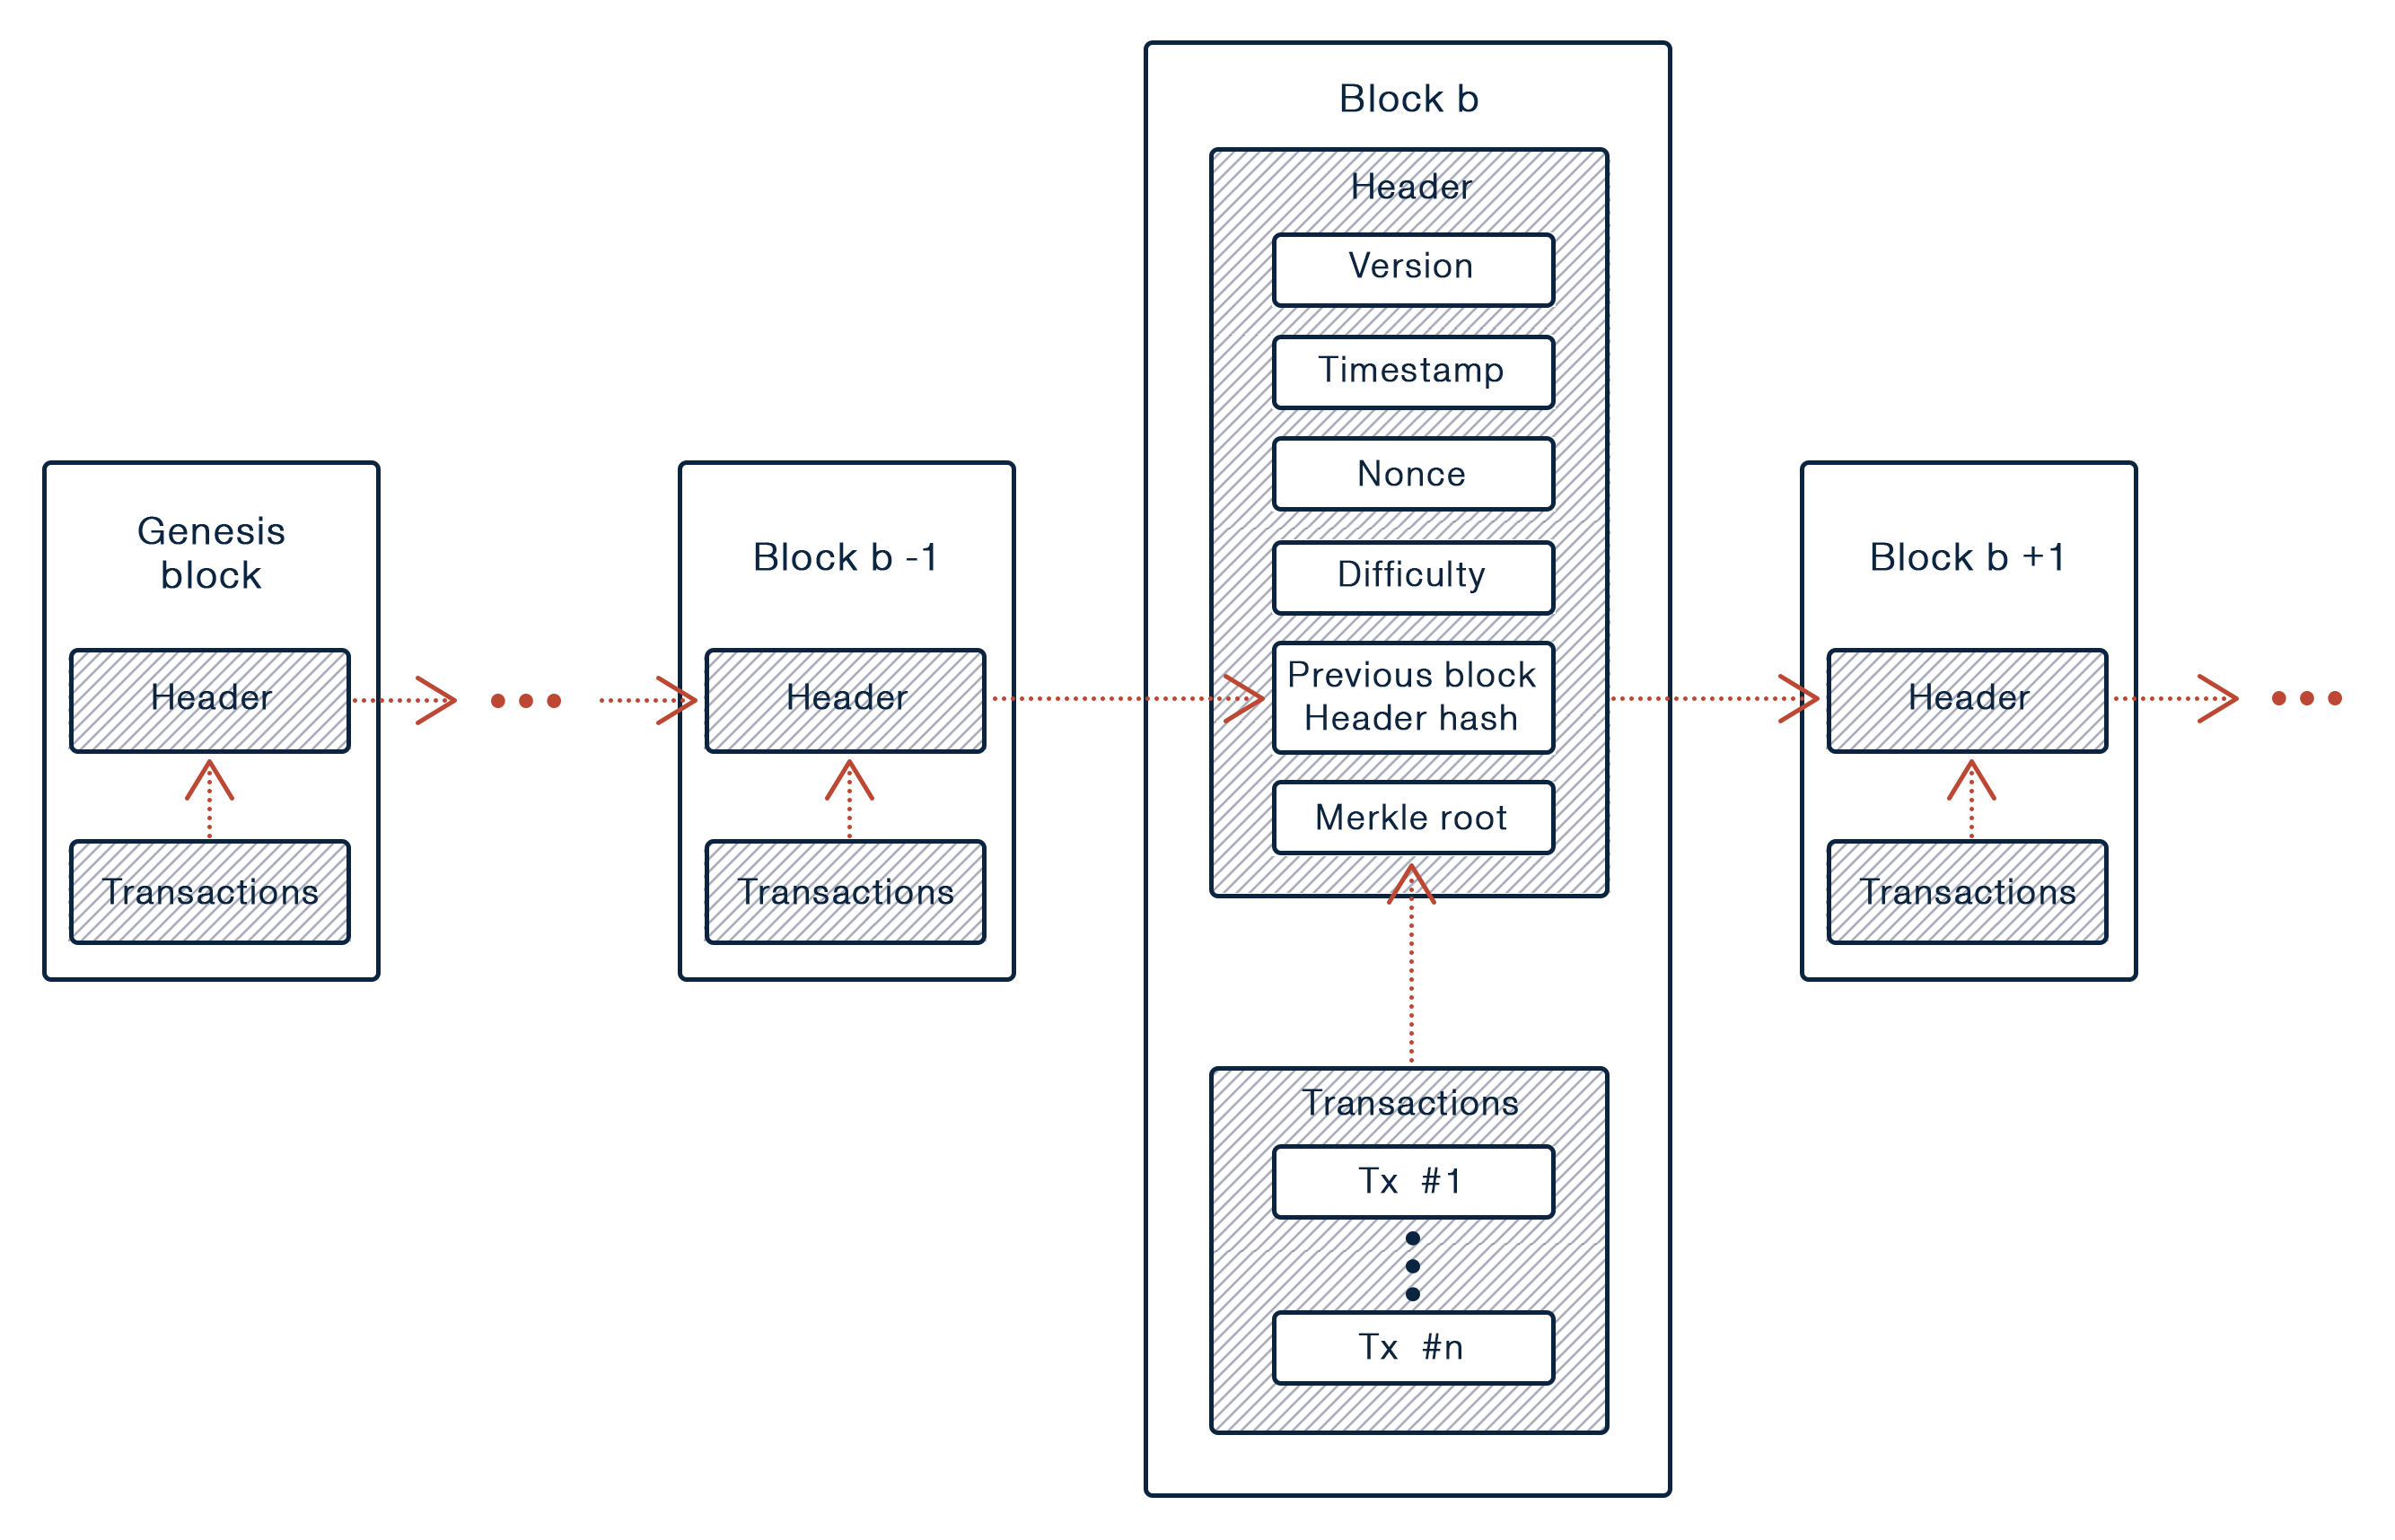
\includegraphics[width=.95\textwidth]{assets/figures/chapter-2/2.3.blockchain}
	\caption{Blockchain ως αλυσίδα από block}
\end{figure}

\vspace{.5\baselineskip}

Ως προς την κυριότητα επί αυτού, το blockchain συνήθως\footnote{Υπάρχουν και κάποιες υλοποιήσεις ιδιωτικών blockchain που, όμως, δε θα μας απασχολήσουν.} δεν ελέγχεται από κάποια κεντρική οντότητα, αλλά διατηρείται από ένα δημόσιο P2P δίκτυο. Οι κόμβοι του δικτύου συμμορφώνονται συλλογικά με ένα πρωτόκολλο συναίνεσης (consensus) για την επικοινωνία και την επικύρωση νέων μπλοκ. Για παράδειγμα, στο Bitcoin, το consensus επιτυγχάνεται μέσω ενός Proof of Work (PoW) αλγορίθμου, όπου οι κόμβοι (miners) ανταγωνίζονται ο ένας τον άλλον για το ποιος θα λύσει πρώτος ένα σύνθετο αλγοριθμικό πρόβλημα που συσχετίζεται με το εκάστοτε block. Αυτός που θα τα καταφέρει επιβραβεύεται για την επεξεργαστική ισχύ που δαπάνησε με ένα ποσό από bitcoin. Εκείνα είναι εν μέρει νέα νομίσματα που κόβονται ή "εξορύσσονται" εκείνη τη στιγμή (όπως ορίζεται από το πρωτόκολλο), αλλά και όσα τέλη (fees) κατέβαλαν οι κόμβοι για να πραγματοποιήσουν τις συναλλαγές του μπλοκ. Αξίζει να σημειωθεί πως δεν είναι αναγκαίο να διαθέτει κανείς ολόκληρο το blockchain (το οποίο είναι ιδιαίτερα ογκώδες) - δηλαδή έναν πλήρη κόμβο - για να επικοινωνήσει με το δίκτυο, αλλά αρκεί να χρησιμοποιήσει έναν light node που απλά να αναμεταδίδει τις επιθυμητές συναλλαγές.

Η διευθυνσιοδότηση σε ένα blockchain επιτυγχάνεται αξιοποιώντας την κρυπτογραφία δημόσιου κλειδιού. Το πρωτόκολλο του εκάστοτε blockchain ορίζει έναν αλγόριθμο για την παραγωγή ζευγών κλειδιών (π.χ. ECDSA στο Bitcoin). Το δημόσιο από αυτά ορίζει τη διεύθυνση, ενώ το ιδιωτικό παραμένει μυστικό, υπό την κατοχή του χρήστη. Με αυτό τον τρόπο προκύπτει ένα πρακτικά ανεξάντλητο πλήθος πιθανών έγκυρων δημόσιων διευθύνσεων (π.χ. $2^{160}$ για το Bitcoin), στις οποίες οι χρήστες μπορούν να στέλνουν και να λαμβάνουν ποσά του εκάστοτε κρυπτονομίσματος. Για την αποστολή ενός ποσού, δηλώνουν το fee που επιθυμούν να καταβάλουν και υπογράφουν την επιθυμητή συναλλαγή με το ιδιωτικό τους κλειδί. Η συναλλαγή αναμεταδίδεται στο δίκτυο και παραμένει στο transaction pool μέχρις ότου να γίνει αποδεκτή και να συμπεριληφθεί στο επόμενο block.

Από τεχνική σκοπιά, το blockchain μπορεί να θεωρηθεί ως μία μηχανή καταστάσεων βασισμένη σε συναλλαγές (transaction-based state machine). Δηλαδή, ξεκινάει από μία αρχική κατάσταση (genesis state), η οποία τροποποιείται σταδιακά με κάθε block, και περιλαμβάνει ανά πάσα στιγμή τις διευθύνσεις με τα ποσά των νομισμάτων που τις αντιστοιχούν.

\begin{figure}[H]
	\centering
	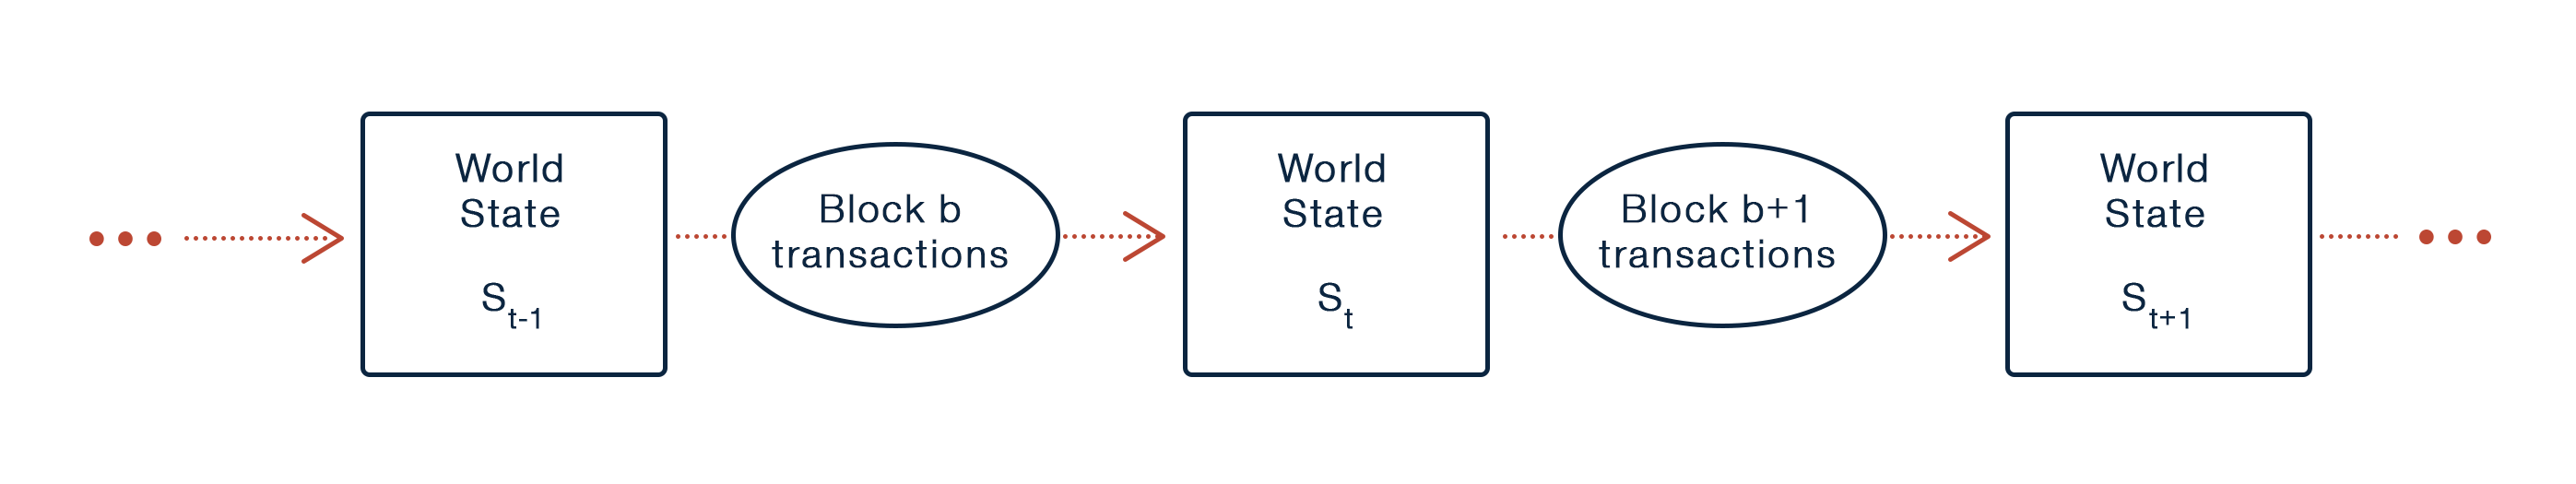
\includegraphics[width=.95\textwidth]{assets/figures/chapter-2/2.3.blockchain.world.state}
	\caption{Blockchain ως μηχανή καταστάσεων}
\end{figure}

Σύμφωνα με την ανάλυση της ενότητας \ref{section:1-2-decentralization}, το blockchain είναι αρχιτεκτονικά και πολιτικά αποκεντρωτικό, καθώς δε διαθέτει δομικά κάποιο κεντρικό σημείο αποτυχίας, ούτε ελέγχεται από κάποιον. Ωστόσο, είναι λογικά συγκεντρωτικό, αφού υπάρχει μία κοινά αποδεκτή κατάσταση και το σύστημα συμπεριφέρεται μακροσκοπικά ως ένας ενιαίος υπολογιστής.
